\lecture{13}{10. Marts 2025}{Composites, Pt. 2 -- Laminates and sandwich panels}

\subsection{Structural composites}
In this course we will focus on two types of structural composites. These are
\begin{itemize}
  \item Laminates
  \item Sandwich Panels
\end{itemize}

\subsubsection{Laminates}
Laminates are created by stacking and bonding multiple layers (laminae) of fiber-reinforces material on top of each other. This can be done in a variety of ways but a common manner of stacking is a \qty{0}{\degree}/\qty{90}{\degree} stacking sequence in which the laminae are stacked such that the fibers are perpendicular to the layer above and below each laminae. This helps achieve a balanced in-plane stiffness and helps mitigate some of the anisotropy that can arise when making composites. Because the fibers in each layer can be oriented differently, laminates can be designed to carry loads efficiently in one or more directions. In general one wants to orient the fibers as much in the direction that will experience stress as possible (multiple stresses from different directions will often require different fiber orientations).

For \qty{0}{\degree} lamina the lamina's stiffness is dominated by the properties of the fibers themselves. The Voigt model (isostrain) typically applies best in this scenario meaning the combined modulus is close to that of the fibers themselves. For \qty{90}{\degree} lamina the matrix carries the most of the load (as the fibers are in the wrong direction). In this case the Reuss model (isostress) best captures the relationship leading to a modulus much closer to that of the matrix itself. For a combination of lamina directions the end result will fall somewhere in-between these two extremes. One can (with reasonable success) approximate the modulus of the composite by using the different rules of mixture (the Reuss and Voigt model) for the respective lamina and then combine the result at the end on basis of the volume fraction or thickness fraction of each lamina direction. 

\subsubsection{Sandwich Panels}
Sandwich Panels consist of a lightweight core (often honeycomb or foam) placed between two stiff, strong face sheets (often made from fiber-reinforced composite or metal). The face sheets carry the bending load, while the core provides shear strength and prevents the face sheets from buckling. This helps achieve a high bending stiffness at a low weight. An adhesive layer is often utilized to secure the face sheets to the honeycomb.

\begin{figure} [ht]
  \centering
  \caption{Illustration of a Sandwich Panel composite}
  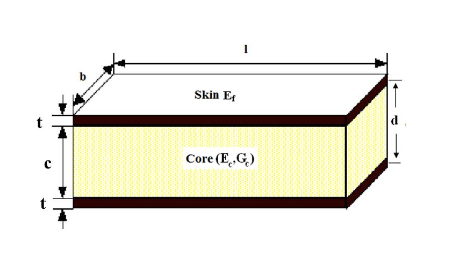
\includegraphics[width=0.75\linewidth]{./figures/f13_1.png}
  \label{fig:f13_1}
\end{figure}
On \textbf{\autoref{fig:f13_1}} an illustration of a Sandwich Panel composite is shown. On this illustration the elastic modulus and shear modulus of the core are labelled $E_c$ and $G_c$ respectively. The thickness of the lamina and the core are $t$ and $c$ respectively. The thickness of the combined composite is $d$, its length is $l$ and its width is $b$. From these we can write some expressions for the material properties of a sandwich panel under bending. The bending stiffness $EI_{eq}$ can be approximated as
\[ 
  EI_{eq} = \underbrace{\frac{E_f b t^3}{6}}_{\text{top face sheet}} + \underbrace{\frac{E_c b c^3}{12}}_{\text{Core}} + \underbrace{\frac{E_f bt d^3}{2}}_{\text{bottom face sheet}}
.\]
In typical Sandwich Panels, the face sheets have a much higher modulus $E_f$ than the core $E_c$ and their thickness $t$ is small compared to the core thickness $c \approx d$. Under these assumptions the dominant term simplifies to:
\[ 
EI_{eq} \approx \frac{E_f bt c^2}{2}
.\]
This indicates that the ost of the bending stiffness comes from the face sheets separated by the thick lightweight core.

The shear stiffness of the Sandwich Panels $AG_{eq}$ can be predicted by
\[ 
AG_{eq} = \frac{b d^2 G_c}{c}
.\]
And because $d \approx c$ this can simplify to
\[ 
AG_{eq} \approx b c G_c
.\]
All in all it is clear that the sandwich panels achieve their high overall stiffness by placing the strong face sheets far apart (large $c$), thereby increasing the moment of inertia for bending, while the core provides shear rigidity.

The deflection of a Sandwich Panel $\delta$ subject to a stress $P$ is the sum of the bending deflection $\delta_b$ and the shear deflection $\delta_s$ as:
\[ 
\delta = \delta_b + \delta_s = \frac{P l^3}{B_1 EI_{eq}} + \frac{P l}{B_2 AG_{eq}}
.\]
Here $B_1$ and $B_2$ are coeffiecients for different loading modes. These coefficients account for boundary conditions (e.g. free vs. built-in ends) and load distributions (point load vs. uniform load). These values can be found in \textbf{\autoref{fig:f13_2}}.

\begin{figure} [ht]
  \centering
  \caption{Coefficients for different loading modes}
  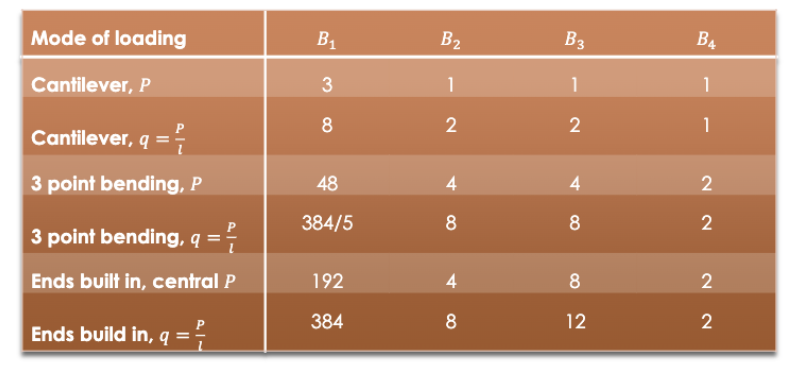
\includegraphics[width=0.5\linewidth]{./figures/f13_2.png}
  \label{fig:f13_2}
\end{figure}

The compliance (the reciprocal of stiffness) can be estimated with the formula:
\[ 
\frac{\delta}{P} = \frac{2 l^3}{B_1 E_f b t c^2} + \frac{1}{B_2 b c G_{c}^{*}}
.\]
Also here are the coefficients from \textbf{\autoref{fig:f13_2}} used.


\begin{exa}[Wind turbine blade]
  A wind turbine blade is exposed to lots of different stresses through its life. The wind exerts a shearing force on the blades and any variation in wind speed or direction will make this shearing force even bigger. On top of this gravity influences the material in a cyclic way meaning the material will be subject to lots of fatiguing stress.

  To combat this one utilizes composites in the wind turbine blades. The aeroshells themselves are made of a sandwich-panel composite. On top of this a load-carrying spear-beam is bonded to the middle of the blade. This spar is often made of a combination of a thick monolithic composite and a sandwich composite. 
\end{exa}
